\documentclass{article}
\usepackage{tikz}
\usetikzlibrary{angles, quotes}
\usepackage{amssymb}
\usepackage{pgfplots}
\pgfplotsset{width=10cm,compat=1.9}
\usepgfplotslibrary{statistics}
\usepackage[left=2.54cm,right=2.54cm,top=2.54cm,bottom=2.54cm]{geometry}
\usepackage{tasks} %Paquete necesario para la producción de items horizontales para algunos ejercicios de tarea empleando el comando /begin{multicols}}{#}.../end{multicols} para ayudarnos a reducir las páginas
\usepackage{pdflscape} %comando que permite cambiar a orientación horizontal las hojas%
\usepackage{soul} %Paquete para permitir la compilación de acentos usando el comando {\hl{}}}\\
\sethlcolor{yellow(munsell)} %comando para definir el color para el subrayado usando el comando \hl
\usepackage[utf8]{inputenc}
\usepackage[spanish]{babel}
\usepackage{icomma}
\usepackage{ragged2e}
\usepackage{siunitx}
\usepackage{url}
\usepackage[colorlinks=true, urlcolor=blue,  linkcolor=black, citecolor=green]{hyperref}
\usepackage{pdfpages}
\usepackage{blindtext} %Paquete que genera texto ficticio (dummy text) con el comando: \blindtext
\usepackage{cancel} %in the preamble gives you four different modes of striking through: \cancel{text to cancel} draws a diagonal line (slash) through its argument, \bcancel{text to cancel} uses the negative slope (a backslash), \xcancel{text to cancel} draws an X (actually \cancel plus \bcancel), \cancelto{〈value〉}{〈expression〉} draws a diagonal arrow through the 〈expression〉pointing to the 〈value〉 (math-mode only)
\usepackage{csquotes}
\usepackage{afterpage}
\usepackage{parskip} 
\usepackage{float}
\usepackage{enumitem}
\usepackage{multicol}%Paquete que permite la creación aislada de columnas de texto. De esta forma se reduce la cantidad de páginas en nuestro documento
\usepackage{lipsum} %Paquete que genera texto de relleno al igual que \usepackage{blindtext}, se usa con el comando \lipsum[#-#] los #(hashtags) delimitan el número de páginas que deseamos ocupar del paquete lipsum para usarlos como relleno. 

% Definir el comando personalizado para la nota
\newcommand{\mynote}[1]{%
\begin{tikzpicture}[baseline=-0.75ex]
	\node[draw, circle, fill=Apple Green!60, inner sep=2pt] (note) {\textbf{Nota:}};
\end{tikzpicture}%
\ \textit{#1}%
}

\newenvironment{Figura}
{\par\medskip\noindent\minipage{\linewidth}}
{\endminipage\par\medskip}
\usepackage{caption}
\usepackage[
backend=biber,
sorting=none,
url=true
]{biblatex} %bibliografía
\addbibresource{biblio.bib}
% Establecer el espacio entre las entradas de la bibliografía
\setlength{\bibitemsep}{1\baselineskip} % Puedes ajustar el valor según tus preferencias
\usepackage{amsmath,amsthm,amssymb,amsfonts}
\usepackage{pifont} %Permite la compilación del comando \xmark: es el símbolo de la tachita
\usepackage{mathtools} %permite la compilación de símbolos para matrices
\usepackage{empheq} %Paquete que se relaciona con \usepackage[most]{tcolorbox} para la creación de cuadros/cajas de colores para delimitar los resultados matemáticos o líneas de texto usando la línea de comando: \begin{empheq}[box={\mymath[colback=orange(webcolor)!70,drop lifted shadow]}]{equation*} \end{empheq}
\usepackage[most]{tcolorbox} %Paquete que se relaciona con \usepackage{empheq} para la creación de cuadros/cajas de colores para delimitar los resultados matemáticos o líneas de texto
\renewcommand{\qedsymbol}{$\blacksquare$}
\usetikzlibrary{positioning,decorations.pathreplacing} %Paquete que permite la compilación de llaves para cuadros sinópticos (brace diagram) 
\usepackage{schemata} %The schemata package is designed just for these brace diagrams
\usepackage{booktabs}

\newcommand\AB[2]{\schema{\schemabox{#1}}{\schemabox{#2}}} %comando o paquete necesario para crear cuadros sinópticos

\newtcbox{\mymath}[1][]{%
nobeforeafter, math upper, tcbox raise base,
enhanced, colframe=blue!30!black,
colback=blue!30, boxrule=1pt,
#1} %Comando importante para encasillar los resultados matemáticos en cajas de diferentes colores, se relaciona con los paquetes \usepackage{empheq} y \usepackage[most]{tcolorbox} 

\newenvironment{sysmatrix}[1]
{\left(\begin{array}{@{}#1@{}}}
{\end{array}\right)}
\newcommand{\ro}[1]{%
\xrightarrow{\mathmakebox[\rowidth]{#1}}%
}
\newlength{\rowidth}% row operation width
\AtBeginDocument{\setlength{\rowidth}{3em}}  %Comando importante para laproducción de lineas de operaciones entre matrices, método de Gauss o Gauss Jordan se relaciona con \newenvironment{sysmatrix}

%formato para cambiar el horario a español
\usepackage[spanish]{datetime2}
\DTMsetdatestyle{spanish}

\renewcommand{\today}{\DTMdisplaydate{\the\year}{\the\month}{\the\day }{-1}}
%%%%%%%%%%%%%%%%%%%%%%%%%%%%%%%%%%%%%%%%%

\usepackage{datetime}
\newcommand{\mycurrenttime}{\xxivtime}

%%%%%%%%%%%%%%%%%%%%%%%%%%%%%%%%%%%%%%%%%%%%%%%%%%%%%%%%%%%%%%%%%%%%%%%%%%%%%%%%%%%%%%%%%%%%%%%%%%%%%%%%%%%%%%%%%%%%%%%%%%%%%%%%%%%%%%%%%%%%%%%%%


%%%%%%%%%%%%%Caja de color para el título%%%%%%%%%%%%%%%%%%%%%%%%%%%%%%%%%%%%%%%%%%%%%%%%%%%%%%

\definecolor{myframecolor}{RGB}{1, 45, 75} % Prussian Blue
\definecolor{myboxcolor}{RGB}{0, 107, 92} % Apple Green

\newtcolorbox{mybox}{
enhanced,
colback=myboxcolor!7, % Color de fondo del cuadro
colframe=myframecolor, % Color del marco del cuadro
arc=0pt,
boxrule=1pt,
borderline west={2mm}{-10mm}{myframecolor}, % Borde en el lado izquierdo
sharp corners=southwest,
width=\linewidth,
before=\par\vspace{\bigskipamount}, % Espacio antes del cuadro
after=\par\vspace{\bigskipamount} % Espacio después del cuadro
}


\newcommand{\euler}{e} %Comando para producir letra e de euler
\newenvironment{remark}{\par\vfill\footnotesize % Vertical white space above the remark and smaller font size
\begin{list}{}{
		\leftmargin=80pt % Indentation on the left
		\rightmargin=60pt}\item\ignorespaces % Indentation on the right
	\makebox[-2.5pt]{\begin{tikzpicture}[overlay]
			\node[draw=Horizon!60,line width=2.5pt,circle,fill=Horizon!25,font=\sffamily\bfseries,inner sep=4pt,outer sep=0pt] at (-19pt,5pt){\textcolor{Horizon}{Nota}};\end{tikzpicture}} % Blue Nota in a circle
	\advance\baselineskip -1pt}{\end{list}\vskip5pt} % Tighter line spacing and white space after remark
	\usepackage{graphicx}
	
	\usepackage{titling}
	
	\input{colores.tex}
	
	%%Producir signos de cita textual``Asignatura''
	
	\newcommand{\xmark}{\ding{55}} %%%comando que genera la tachita
	
	\newenvironment{MyColorPar}[1]{%
\leavevmode\color{#1}\ignorespaces%
}{%
}%

%%%%%%%%%%%%%%%%%%% Título de la tarea, Nombre de alumno

\title{ \textcolor{Tarawera}{\textbf{T-\textcolor{Sun}{\textbf{14}}}}: \textcolor{Cinnabar}{\textbf{Transcripción de notas (\underline{Cap 5}): \textcolor{orange(colorwheel)}{\textbf{Aprender y enseñar ciencia. Del conocimiento cotidiano al conocimiento científico$^{ \textcolor{trueblue}{\text{J. I. Pozo; M. A. Gómez Crespo}} }$    }}}}}
\author{\emph{Julio Alfredo Ballinas García} $\boldsymbol{\mid}$ 202107583}
\date{\today}

%%%%%%%%%%%%%%%%%%% Datos de la Materia

\usepackage{fancyhdr}
\fancypagestyle{plain}{%  the preset of fancyhdr 
\fancyhf{} % clear all header and footer fields
\fancyfoot[R]{
\includegraphics[width=2cm]{LogoFCFMBUAP (1).png}}
\fancyfoot[L]{{\bfseries{\thedate{}}} a las {\bfseries{\mycurrenttime{}}} horas{} (GMT-6, H. Puebla de Zaragoza, Pue)}
\fancyhead[L]{Enseñanza de la física }
\fancyhead[R]{\theauthor}
}
\makeatletter
\def\@maketitle{%
\newpage
\null
\vskip 1em%
\begin{center}%
	\let \footnote \thanks
	{\LARGE \@title \par}%
	\vskip 1em%
	%{\large \@date}%
\end{center}%
\par
\vskip 1em}
\makeatother

\usepackage{lipsum}  
\usepackage{cmbright}


%%%%%%%%%%%%%%%%%%%%%%%%%%%%%%%%%%%%%%%%%%%%%%%%%%%%%%%%%%%%%%%%%%%%%%%%%%%%%%%%%%%%%%%%%%%%%%%%%%%%%%%%%%%%%%%%%%%%%%%%%%%%%%%%%%%%%%%%%%%%%%%%%%%%%%%%%%%%%%%%%%%%%%%%%%%%%%%%%%%%%%%%%%%%%%%%%%%%%%

\begin{document}



\maketitle


%%%%%%%%%%%%%%%%%%% Datos del profesor, campus y aula

\begin{mybox}
  \noindent\begin{tabular}{@{}ll}
    {\bfseries{Profesor}} & Dr. Apolonio Juárez Nuñez\\
    \textcolor{prussianblue}{\bfseries{Campus}} / \textcolor{trueblue}{\bfseries{Facultad}}  & \textcolor{prussianblue}{\bfseries{C.U. BUAP}} /  \textcolor{trueblue}{\bfseries{FCFM}} \\
    \textcolor{prussianblue}{\bfseries{Edificio}} /  \textcolor{trueblue}{\bfseries{Salón}}    &   \textcolor{prussianblue}{\bfseries{1FM4}} /  \textcolor{trueblue}{\bfseries{104}}   
  \end{tabular} 
\end{mybox} \vspace{1cm}

\section*{Instrucciones de la actividad}
\addcontentsline{toc}{section}{Instrucciones de la actividad}

\setlength{\columnsep}{2cm}
\begin{multicols}{2}

\begin{enumerate}[label={{\textcolor{trueblue}{\textbf{Ej}. \arabic*.0}}}, start=1]
  \item \textbf{De este texto:} \emph{Aprender y enseñar ciencia. Del conocimiento cotidiano al conocimiento científico} (\underline{Capítulo 5}).\\[4pt]
        Elaborar una lista con \textbf{20 ideas principales}
        \begin{enumerate}[label=\alph*)]
          \item Cada idea debe corresponder a un fragmento o afirmación relevante del texto.
        \end{enumerate}
\end{enumerate}

\end{multicols}

\vspace{2cm}






\tableofcontents  \vspace{2cm}


\section*{\textcolor{Tarawera}{ \textbf{ \textcolor{Mantle}{\textbf{Cap V:}} Del conocimiento cotidiano al conocimiento científico: más allá del cambio conceptual}}}
\addcontentsline{toc}{section}{\textcolor{Tarawera}{ \textbf{ \textcolor{Mantle}{\textbf{Cap V:}} Del conocimiento cotidiano al conocimiento científico: más allá del cambio conceptual}}}


\subsection*{La hipótesis de la compatibilidad o la acumulación de saberes}
\addcontentsline{toc}{subsection}{La hipótesis de la compatibilidad o la acumulación de saberes}

\begin{enumerate}
  \setcounter{enumi}{0}

  \item
  \begin{quote}
  Una primera interpretación es que los procesos y productos del conocimiento cotidiano y científico tienen básicamente la misma naturaleza, que las personas de la calle y los científicos piensan esencialmente igual cuando se enfrentan a un problema. Por decirlo de un modo gráfico, ahora que las tecnologías de la información son inevitablemente la metáfora de nuestro modo de conocer y aprender (\textsc{Pozo}, 1996a), la mente del científico y la de la persona de la calle (incluidos los alumnos) estarían \textit{formateadas} de la misma manera, de modo que los programas que corren en una y otra serían compatibles. \hl{(p.~130–131)}
  \end{quote}

  \item
  \begin{quote}
  ¿A qué se deberían entonces las diferencias tan obvias entre los productos del conocimiento cotidiano (las llamadas concepciones alternativas, caracterizadas en el capítulo anterior) y del conocimiento científico (las teorías y modelos que son objeto de enseñanza)? No tendrían tanto un origen intelectual o cognitivo, como social y cultural. La ciencia es una tarea acumulativa que se produce en determinados contextos sociales y culturales, de forma que el alumno carecería de los saberes y las actitudes necesarios para incorporarse a esa tarea cultural. Así, desde esta perspectiva, el cambio conceptual no sería necesario, ya que aprender ciencia sería sobre todo un proceso de acumulación de saberes y experiencias y no tanto un proceso de reorganizar, o reformatear, la mente de los alumnos por procesos de cambio conceptual. \hl{(p.~131)}
  \end{quote}
\end{enumerate}


\subsection*{La hipótesis de la incompatibilidad o el cambio conceptual}
\addcontentsline{toc}{subsection}{La hipótesis de la incompatibilidad o el cambio conceptual}

\begin{enumerate}
  \setcounter{enumi}{2}

  \item
  \begin{quote}
  La mayor parte de la investigación reciente en aprendizaje y enseñanza de las ciencias, basada en el enfoque de las concepciones alternativas (resumida y analizada en el capítulo anterior), asume de hecho que, en contra de la hipótesis anterior, la mente del científico y la del alumno tienen en algún sentido formatos incompatibles, que usan lenguajes diferentes, o incluso, utilizando la terminología de \textsc{Kuhn} (1962), que son hasta cierto punto \textit{inconmensurables}, no se pueden reducir ni traducir la una a la otra. En otras palabras, para que los alumnos aprendan las teorías y modelos científicos, es preciso que cambien radicalmente su forma de interpretar las cosas, ya que de lo contrario, como sucede habitualmente, tenderán a cometer errores conceptuales, \textit{misconceptions}, a malinterpretar lo que estudian, asimilándolo a sus propias concepciones alternativas. [...] Es preciso cambiar a través de la enseñanza los conocimientos previos que trae el alumno y acercarle a los conocimientos científicos. \hl{(p.~134–135)}
  \end{quote}

  \item
  \begin{quote}
  Como veremos en el Capítulo VIII buena parte de las estrategias didácticas diseñadas teniendo en cuenta los conocimientos previos de los alumnos han estado dirigidas de modo explícito o implícito a \textit{sustituir}, a cambiar esos conocimientos, incompatibles con los marcos conceptuales de la ciencia, por otros más próximos a las teorías científicas aceptadas. [...] En las contundentes palabras de \textsc{Duit} (1999) “hay que afirmar que no hay ni un solo estudio en la literatura de investigación sobre las concepciones de los estudiantes en el que una concepción concreta de las que están profundamente arraigadas en los alumnos haya sido totalmente extinguida y sustituida por una nueva idea”. La mayoría de las investigaciones muestran que hay sólo un éxito limitado en relación con la aceptación de las ideas nuevas y que las viejas ideas siguen básicamente “vivas” en contextos particulares. \hl{(p.~135–136)}
  \end{quote}
\end{enumerate}


\subsection*{La hipótesis de la independencia o el uso del conocimiento según el contexto}
\addcontentsline{toc}{subsection}{La hipótesis de la independencia o el uso del conocimiento según el contexto}

\begin{enumerate}
  \setcounter{enumi}{4}

  \item
  \begin{quote}
  Frente a la concepción dominante, al menos implícitamente, en el enfoque de las concepciones alternativas, que fijaba como meta educativa el rechazo por parte del alumno de sus concepciones alternativas, que se consideraban erróneas e inferiores a las científicas, por las que debían ser “cambiadas”, en los últimos años han venido cobrando importancia las posiciones que defienden la necesidad de que la persona disponga de diferentes representaciones o modelos para enfrentarse a distintas tareas. En lugar de pretender que el alumno abandone su mecánica intuitiva para asumir los modelos de la física newtoniana, se trataría de que logre diferenciar entre ambos modelos y aprenda a usarlos discriminativamente en función del contexto. [...] Igualmente, los modelos de conocimiento o aprendizaje “situado” destacan la necesidad de analizar el funcionamiento intelectual en el contexto de las demandas de las tareas, habiéndose alcanzado también la idea de cambio conceptual contextual. \hl{(p.~137–138)}
  \end{quote}

  \item
  \begin{quote}
  En suma, todos los sujetos dispondrían de hecho de representaciones alternativas para un mismo hecho que activarían de modo más o menos discriminativo, en función del contexto, por lo que el objetivo de la educación científica no debería ser en ningún caso erradicar o extinguir las concepciones alternativas de los alumnos, sino más bien separar ambas formas de conocimiento, de que los sujetos aprendieran a utilizarlas en contextos diferentes. [...] Como ha argumentado \textsc{Claxton} (1991), la fe en el carácter automático y necesario de esa transferencia —la idea de que el conocimiento científico es útil en todos los contextos— está en la base de las metas de la mayoría de los currículos de “ciencia para todos”. Sin embargo, parece claro que, aunque el conocimiento científico deba ser utilizado en todos los ámbitos, la meta de la educación debe ser precisamente \textit{descontextualizar}, hacer más transferible y generalizable el conocimiento. \hl{(p.~138–139)}
  \end{quote}
\end{enumerate}


\subsection*{La hipótesis de la integración jerárquica o los diferentes niveles de representación y conocimiento}
\addcontentsline{toc}{subsection}{La hipótesis de la integración jerárquica o los diferentes niveles de representación y conocimiento}

\begin{enumerate}
  \setcounter{enumi}{6}

  \item
  \begin{quote}
  Según esta hipótesis, la activación contextual de teorías alternativas no es incompatible con la necesidad del cambio conceptual entendido como la construcción del conocimiento científico a partir del cotidiano. [...] En lugar de pretender separar o independizar ambas teorías, la científica y la cotidiana, según la hipótesis de la integración jerárquica se trataría de conectarlas mediante procesos metacognitivos, de convertir en objeto de reflexión las diferencias entre ambas teorías, de forma que puedan ser integradas como distintos niveles de análisis o de complejidad en la interpretación de un problema. \hl{(p.~140)}
  \end{quote}

  \item
  \begin{quote}
  Por ello, aunque las teorías científicas tienen una mayor potencia explicativa, un exceso de contenido empírico con respecto al conocimiento cotidiano no las hace innecesarias. [...] En suma, la teoría intuitiva, aunque desde el punto de vista conceptual pudiera ser subsumida por la teoría científica, desde el punto de vista del procesamiento seguiría siendo eficaz en los contextos informales cotidianos. [...] Esta idea del aprendizaje de la ciencia, entendido como la integración jerárquica de modelos, implica por tanto diferentes procesos de construcción del conocimiento científico que van más allá del cambio conceptual tal como habitualmente se ha entendido. \hl{(p.~141–142)}
  \end{quote}
\end{enumerate}


\subsection*{Los procesos de construcción del conocimiento científico}
\addcontentsline{toc}{subsection}{Los procesos de construcción del conocimiento científico}

\begin{enumerate}
  \setcounter{enumi}{8}

  \item
  \begin{quote}
  A partir de las diversas teorías sobre la construcción del conocimiento científico en contextos escolares desde el conocimiento cotidiano (por ejemplo, \textsc{Chi}, 1992; \textsc{Glynn y Duit}, 1995b; \textsc{Lawson}, 1994; \textsc{Pozo}, 1996a, 1997a; \textsc{Rodrigo y Correa}, 1999; \textsc{Vosniadou}, 1994a), y sobre todo de los análisis presentados en los dos últimos capítulos sobre las relaciones entre el conocimiento cotidiano y el científico, podemos identificar tres procesos fundamentales en la construcción del conocimiento científico en el aula. Estos procesos, reflejados en la Figura~\ref{fig:figura_5_1}, serían la reestructuración teórica, la explicitación progresiva y la integración jerárquica de las teorías implícitas de los alumnos en las teorías científicas. Aunque esos tres procesos, como vamos a ver, están estrechamente vinculados entre sí, analizaremos cada uno de ellos por separado. \hl{(p.~142)}
  \end{quote}
\end{enumerate}

\begin{figure}[H]
  \centering
  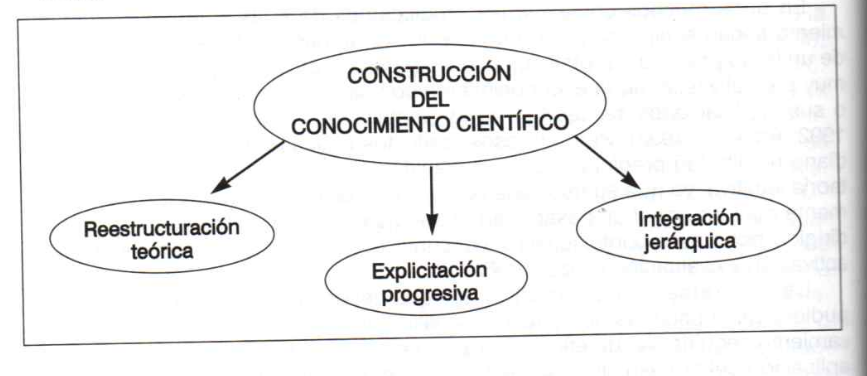
\includegraphics[width=0.65\textwidth]{figura_5_1.png}
  \caption{Procesos fundamentales en la construcción del conocimiento científico en el aula.}
  \label{fig:figura_5_1}
\end{figure}

 
\subsection*{El proceso de reestructuración}
\addcontentsline{toc}{subsection}{El proceso de reestructuración}

\begin{enumerate}
  \setcounter{enumi}{9}

  \item
  \begin{quote}
  La \textit{reestructuración} implica construir una nueva forma de organizar el conocimiento en un dominio que resulte incompatible con las estructuras anteriores. Según la interpretación que hemos hecho en páginas precedentes, ese cambio conceptual o reestructuración será necesario cuando la superación de las teorías alternativas en un dominio dado requiera adoptar nuevos supuestos epistemológicos, ontológicos y conceptuales desde los que interpretar los escenarios y situaciones en ese dominio. \hl{(p.~142–143)}
  \end{quote}

  \item
  \begin{quote}
  En concreto, la reestructuración deberá traducirse y concretarse en un cambio de las estructuras conceptuales utilizadas en un dominio de conocimiento dado, desde las formas más simples propias del conocimiento cotidiano hasta las estructuras más complejas de las teorías científicas. [...] En otras palabras, los contenidos de la educación científica deben seguir siendo los conceptos, técnicas, estrategias, actitudes, etc., que constituyen el saber científico, pero la meta de la enseñanza de esos contenidos debería ser promover cambios más profundos en las estructuras conceptuales, los valores o el saber estratégico. \hl{(p.~143–144)}
  \end{quote}

  \item
  \begin{quote}
  En el caso de los contenidos conceptuales se trataría de que, partiendo del estudio de nociones concretas, el alumno vaya haciendo explícitos los supuestos en los que basa sus interpretaciones y, al hacerlo, profundice en las estructuras conceptuales que subyacen a sus predicciones, acciones y creencias. El proceso de reestructuración requiere por tanto una explicitación progresiva de las teorías implícitas del alumno. \hl{(p.~144)}
  \end{quote}
\end{enumerate}


\subsection*{El proceso de explicitación progresiva}
\addcontentsline{toc}{subsection}{El proceso de explicitación progresiva}

\begin{enumerate}
  \setcounter{enumi}{12}

  \item
  \begin{quote}
  La construcción del conocimiento científico implica también un proceso metacognitivo, o aun mejor metaconceptual, de \textit{explicitación} de las concepciones mantenidas intuitivamente. [...] Será necesario, con el fin de promover el cambio conceptual, diseñar escenarios que faciliten ese proceso de explicitación, enfrentando al alumno a problemas potenciales a ser posible en contextos de interacción social que induzcan la comunicación de las propias concepciones. \hl{(p.~144)}
  \end{quote}

  \item
  \begin{quote}
  La tarea metacognitiva consistiría en un proceso de hacer explícitos de forma progresiva algunos de esos supuestos, con el fin de poder cambiarlos, partiendo del nivel más superficial hacia niveles representacionales cada vez más profundos. Además de este proceso de profundización en los niveles representacionales, la explicitación progresiva tiene una segunda dimensión esencial, la \textit{formalización} de las representaciones en códigos o lenguajes cada vez más explícitos. \hl{(p.~145)}
  \end{quote}

  \item
  \begin{quote}
  De esta forma, la explicitación, a medida que profundiza en las representaciones y las formaliza, favorecerá los procesos de reestructuración, al permitir al alumno tomar conciencia de las diferencias estructurales y conceptuales entre las teorías científicas y sus propias teorías. [...] El cambio conceptual suele implicar un proceso de \textit{integración jerárquica}, por el que las formas de representación más elementales se integran, o se redescubren, en las más complejas. \hl{(p.~145)}
  \end{quote}
\end{enumerate}

\subsection*{El proceso de integración jerárquica}
\addcontentsline{toc}{subsection}{El proceso de integración jerárquica}

\begin{enumerate}
  \setcounter{enumi}{15}

  \item 
  \begin{quote}
  Cualquier situación o fenómeno científico sería susceptible de ser analizado, o representado, desde diferentes teorías alternativas, que implicarían distintos niveles de análisis, basados en estructuras conceptuales de complejidad diversa. [...] Las teorías alternativas suelen ser muy predictivas en contextos cotidianos, además de aplicarse con una gran economía de recursos cognitivos, dada su naturaleza implícita. \hl{(p.~145–146)}
  \end{quote}

  \item
  \begin{quote}
  De esta forma la teoría intuitiva, aunque desde el punto de vista conceptual pudiera ser subsumida por la teoría científica, desde el punto de vista del procesamiento seguiría siendo eficaz en los contextos informales cotidianos. [...] Sin embargo, una adecuada integración jerárquica entre los modelos permitiría utilizar una \textit{high road} o vía de alto nivel al discriminar metacognitivamente entre diferentes niveles representacionales. \hl{(p.~146)}
  \end{quote}

  \item
  \begin{quote}
  En general, puede asumirse que una teoría es más potente, y permite integrar a otra más simple parcial o totalmente, cuando: (a) tiene una mayor capacidad de generalización; (b) tiene una estructura conceptual más compleja; (c) tiene mayor poder explicativo o de redescription representacional. \hl{(p.~146)}
  \end{quote}

  \item
  \begin{quote}
  En suma, la construcción del conocimiento científico requiere construir estructuras conceptuales más complejas a partir de otras más simples y, probablemente, establecer usos diferenciales para cada uno de los contextos de aplicación de esas teorías. [...] Las teorías científicas, al implicar una toma de conciencia y explicitación de las relaciones entre los modelos interpretativos, proporcionan la ciencia y sus propias concepciones alternativas. \hl{(p.~146–147)}
  \end{quote}

  \item
  \begin{quote}
  Todo este proceso de reestructuración, explicitación e integración jerárquica debe ir, como hemos señalado en más de una ocasión, \textit{de abajo hacia arriba}, desde los niveles representacionales más superficiales a los más profundos, de los escenarios concretos a las estructuras de los hechos, de los hechos a los conceptos y de los conceptos a los principios. \hl{(p.~147)}
  \end{quote}
\end{enumerate}


\end{document}
